% !TEX program = pdflatex
% ============================================================
% Optics Express manuscript -- generated from manuscript_draft.md by md2optica.py
% Requires opticajournal.cls (not distributable; see README.md)
% ============================================================
\documentclass[9pt,twocolumn,twoside]{opticajournal}
\journal{opticajournal}   % Optics Express uses the opticajournal layout
\usepackage{lineno}
\linenumbers

\begin{document}

\title{Practical Saturation of Freeform Microlens Arrays on Extended OLED Emitters and Design Routes beyond Lens Shape}

% ---- authors: fill in ----
\author{Author One\authormark{1}, Author Two\authormark{1} and Author Three\authormark{1,*}}
\address{\authormark{1}[Affiliation, Address]\\}
\email{\authormark{*}[corresponding@email]}


\begin{abstract*}
Freeform microlens arrays (MLAs) and numerical inverse design are widely expected to give simultaneous control over the light-extraction efficiency and the angular emission profile of organic light-emitting diodes (OLEDs). This expectation, however, largely originates in illumination optics built around point-like sources far smaller than the lens aperture, and it does not automatically transfer to an MLA tiled coextensively over a uniform, extended emitter. Here we combine a dipole microcavity source model based on the classical power spectrum (CPS) formalism with three-dimensional ray tracing to compare hemispherical reference lenses and axisymmetric freeform lenses under identical geometric, material, and process constraints, supplemented by a separately constrained asymmetric, off-axis freeform exploration. Total external quantum efficiency (EQE) and each of the four polar bands (0–20\ensuremath{^\circ}, 20–40\ensuremath{^\circ}, 40–60\ensuremath{^\circ}, 60–80\ensuremath{^\circ}) were optimized as independent single objectives, complemented by a weighted-sum sweep between total EQE and the 40–60\ensuremath{^\circ} band. Against a hemispherical reference optimized under the same constraints, the best freeform design exceeds the hemisphere by at most 7\% in any polar objective and by 1.3\% in total EQE, and never falls below it. Restarting each search at the hemispherical optimum confirms that the two bands where a randomly seeded search had fallen short were search artifacts: the deficit is recovered and the residual gain is at most +0.3\%—a five-repeat re-measurement resolves it as statistically real ($t = 4.1$) yet practically negligible—while the identical procedure recovers margins of +1.0\% to +4.7\%, at significances of $t = 30$ to $115$, in the three objectives where they genuinely exist. Across 150 randomly sampled feasible designs and all optimized designs, spanning total EQE from 0.12 to 0.56, the (total EQE, band EQE) points collapse onto a single near-linear frontier: efficiency and band power rise together, and no efficiency-versus-directionality trade-off is observed. Among the twenty most efficient designs the band selectivity is nearly invariant—its 10–90\% spread is 0.092–0.096, 0.277–0.281, 0.358–0.364 and 0.233–0.238 for the four bands—even though these designs were located by four different objectives. Dedicating the objective to a single band does move the distribution: selectivity rises by up to 27\% (0–20\ensuremath{^\circ}) and 20\% (60–80\ensuremath{^\circ}) above that natural spread. The gain is not free, however, as the same designs give up to 11\% of total extraction, so the net band power of a band-dedicated optimum exceeds the best design found while pursuing any other objective by at most 6\% in every band. Beyond this benchmark family, we stress-test two further manufacturable external-film MLA families—an inverted (concave) MLA and a randomly assembled MLA represented by a pseudo-random supercell—under the same protocol. The inverted family reproduces every signature at 6\% lower total extraction, and its largest steering budget, 1.19 in the 60–80\ensuremath{^\circ} band, matches the convex value of 1.20 obtained in a different band. Its natural composition shifts slightly relative to the convex one under identical patch size, source and stack (0.113/0.303/0.340/0.215 versus 0.094/0.278/0.361/0.236), by an amount comparable to the difference between two reasonable ways of averaging within a single family. The randomly assembled family lands inside the same window despite randomised lenslet positions and an independently drawn profile for every lenslet, and is insensitive to the particular disorder realisation (0.2\% coefficient of variation across three seeds). Across all three constructions and both averaging conventions, every high-efficiency composition falls within 0.09–0.11 / 0.28–0.30 / 0.34–0.36 / 0.21–0.24. The angular composition is therefore a property of the platform—extended source, thick substrate, coextensive external film—rather than a design variable that shape freedom, array construction, or disorder can command.

We explain this practical saturation by three factors. First, in a coextensively tiled array the lens aperture and the effective source patch grow in the same proportion, so the area leverage that underlies point-source collimation does not arise. Second, lateral propagation in the substrate mixes light between neighboring lenslets and erases the spatial information a local surface shape could exploit. Third, a passive external layer operating on a given source radiance and exit area faces a practical ceiling on the power it can deliver into a chosen angular channel. These results do not render freeform MLAs meaningless; across the three tested manufacturable external-film families they provide a quantitative criterion for deciding when further investment in shape complexity on extended OLEDs should stop. Finally, we organize the three routes that remain productive after MLA saturation—source/cavity engineering, aperture expansion, and angular-selective recycling—in the same physical language, and present a design-route map for choosing the next lever. In an idealized recycling model with 10\% round-trip loss, an angular filter delivers 62.1\% of the generated power into the 40–60\ensuremath{^\circ} band, whereas the planar non-selective reference stays at 29.1\%; a realizable eight-pair dielectric multilayer reaches 48.2\% for a monochromatic source but degrades to 32.5\% over a 100 nm bandwidth, identifying source bandwidth and loss as the practical constraints of this route.
\end{abstract*}


\section{1. Introduction}

External light extraction remains a central limit on the efficiency and high-luminance lifetime of OLEDs. Waveguided modes in the organic layers, loss channels associated with the metal electrode, and total internal reflection at the substrate/air interface together trap a large fraction of the photons generated in a planar OLED \cite{r1,r2}. External MLAs can extract the substrate modes without perturbing the electrical structure of the device, and have therefore been an attractive solution for large-area and flexible OLEDs in particular \cite{r3,r4,r5}. Hemispherical or near-hemispherical MLAs already reach high efficiencies, and very high EQE has been reported for OLEDs with embedded hemispherical MLAs \cite{r4,r5}.

Nevertheless, the expectation attached to more complex shapes persists. Freeform illumination optics and inverse design are powerful tools for producing prescribed intensity distributions, and have recently been applied to the optical packaging of micro-LEDs and OLEDs \cite{r6,r7}. Intuitively, tuning the asymmetry, curvature distribution, height, pitch, or the microcavity condition of the lenses simultaneously should offer finer control over total extraction and over emission into specific directions than a hemispherical MLA does.

Two observations sharpen this intuition into a testable question. On one hand, freeform design methods were largely developed for sources of near-zero étendue, whereas a thin-film emitter is an extended source whose light reaches the array only after propagation, and partial recycling, inside the substrate. On the other hand, high total extraction demonstrably does not require lenses at all: Song et al. reported lens-free OLEDs exceeding 50\% EQE using an external random scattering layer combined with horizontally oriented emitters \cite{r13}. If total efficiency is reachable without shaped surfaces, the question that remains—and the one this paper addresses—is whether freeform lens shape buys angular control \emph{on top of} efficiency on an extended emitter.

This question matters in practice. Freeform design and precision molding raise fabrication cost and metrology burden; if the achievable gain barely exceeds a hemispherical reference, the next design step should not be a more complex surface but a change of source, aperture, or recycling path. Our aim is therefore not "can a better freeform lens be found?" but: \textbf{how much is shape freedom actually worth for a tiled refractive MLA on an extended OLED?}

We compare, under one OLED source model previously validated against fabricated devices \cite{r16,r17} and one set of manufacturable geometric constraints, (i) a hemispherical MLA and (ii) an axisymmetric freeform MLA, and we additionally examine (iii) an asymmetric three-dimensional freeform exploration performed as a separate, differently constrained study (Section 2.4). We further probe the generality of the outcome on two additional manufacturable external-film MLA families—inverted and randomly assembled arrays (Section 2.5). We use total EQE and polar-band EQE as independent objectives, employ surrogate-based multi-start optimization with high-precision re-evaluation to separate optimizer dependence from physics, and connect the outcome to a radiance/étendue picture and to lateral mixing in the substrate. We emphasize the epistemic status of the result throughout: it is not an impossibility theorem but a reproducible numerical observation—\textbf{a practical saturation of the explored freeform design space}—together with a quantitative account of why it occurs and of which optical levers remain productive beyond it.

\section{2. Results and Discussion}

\subsection{2.1 A fairly aligned benchmark: isolating the effect of shape complexity itself}

Fig.~\ref{fig:1} shows the optical system under comparison. Dipole emission in the OLED microcavity is computed with the CPS formalism to obtain the substrate-side angular–spectral distribution $I_{\mathrm{sub}}(\theta,\lambda)$, which serves as the source for three-dimensional ray tracing. The emitting region is a disc of radius $r_{\mathrm{OLED}} = 1$ mm on a substrate of thickness $d_{\mathrm{sub}} = 1.295$ mm; the exit face carries a two-dimensional hexagonal array of lenslets of approximately 10 \ensuremath{\mu}m radius extending over 25 \ensuremath{\times} 25 mm, so that laterally spreading substrate light remains within the array. The source is thus extended by two orders of magnitude relative to an individual lenslet—the regime of interest for tiled outcoupling films. All lenses satisfy the same substrate index, lens material, pitch, fill factor, maximum height, and maximum draft-angle constraints. Cavity thicknesses are co-optimized with the lens in every campaign, so each lens class is compared at its own best cavity rather than at a shared one.

This alignment is essential. If the freeform class were allowed a wider variable range, a greater lens height, a larger aperture, or a more favorable cavity, shape effects would be confounded with other effects. Here the hemispherical MLA is itself optimized over the same outer radius and the same manufacturable height range, and the freeform class is subject to constraints that are identical—never more permissive. Subsequent performance differences can therefore be read, as far as possible, as the pure effect of shape freedom.

\begin{figure*}[t]
\centering

\includegraphics[width=\textwidth]{figures/fig1_platform.pdf}
\caption{\textbf{Platform and benchmark design.} (a) OLED–substrate–MLA architecture: CPS microcavity dipole source ($r_{\mathrm{OLED}} = 1$ mm), glass substrate ($d_{\mathrm{sub}} = 1.295$ mm), hexagonal lenslet array (\ensuremath{\sim}10 \ensuremath{\mu}m lens radius, 25 \ensuremath{\times} 25 mm extent). (b) The two lens classes under identical constraints, drawn to the same scale in units of the lens radius: the hemispherical reference (3 free variables) and the axisymmetric freeform (13 variables); open circles are the five free spline control points, with the endpoints fixed at (0,1) and (1,0). The freeform shown is the 40–60\ensuremath{^\circ} optimum. (c) Definition of the four polar bands and of the band selectivity $S_j$, taken over the full azimuth. (d) Optimization workflow: CPS source, LightTools ray tracing driven over the MATLAB COM interface, surrogate-based global search, pattern-search polishing, and high-ray re-evaluation.}
\label{fig:1}
\end{figure*}


\subsection{2.2 Changing the objective does not carry designs far beyond the hemispherical reference}

Fig.~\ref{fig:2}d,e summarizes the best attained performance when total EQE and individual polar bands are maximized. For each objective $j$ we define the relative gain

\begin{equation}
G_j=\frac{\max\left[\mathrm{EQE}_j\mid\mathrm{freeform}\right]}
{\max\left[\mathrm{EQE}_j\mid\mathrm{hemisphere}\right]},
\end{equation}

where each maximum is defined after independent initializations, multiple starts, and high-ray re-evaluation, as the mean of the re-evaluated repeats. The hemispherical reference was optimized under the same constraints, stack, patch and fidelity, with its five profile control points fixed on a quarter circle and its cavity thicknesses and lens height left free. Across the four polar objectives $G_j$ = 1.003, 1.002, 1.070 and 1.036, and for total EQE $G$ = 1.013. The total-EQE numerator comes from the campaign dedicated to that objective, which reaches 0.5539 over three independent starts (0.8\% spread across starts) at the fixed 25 \ensuremath{\times} 25 mm patch; the hemisphere-seeded control independently reaches 0.5523 in the same session as the hemisphere baseline of 0.54679, so the freeform ceiling at the fixed patch is located twice, by different procedures, 0.3\% apart. The weighted-sweep campaign's higher total of 0.5556 is not a competing value but a different normalization: re-measuring that campaign's best design at the fixed patch gives 0.5428, while at a 100 mm patch the same design gives 0.5636. The archived 0.5556 falls between the measured 35 mm and 100 mm values, consistent with a larger effective patch having been in force when that campaign ran (Section 2.6; Supplementary Table S7). Its absolute values are therefore not compared directly against the fixed-patch hemisphere. The freeform optimum never exceeds an equally optimized hemisphere by more than 7\% in any objective, and never falls below it. The freeform optimum therefore never exceeds an equally optimized hemisphere by more than 7\% in any objective, and exceeds it by 1.6\% in total extraction.

Reaching those numbers required a control that we report in full, because the first version of this comparison did not pass it. In the original per-band campaign, seeded randomly, the 0–20\ensuremath{^\circ} and 20–40\ensuremath{^\circ} gains came out \emph{below} unity, at 0.946 and 0.966. That is impossible as a statement about optics—the hemisphere is itself a point of the 13-parameter feasible set, so $G_j \ge 1$ by construction with unlimited budget—and it is therefore a statement about search. It is also the strongest available objection to everything that follows: a search that fails to recover a solution it contains cannot be trusted when it reports that nothing better exists.

We removed the ambiguity by restarting each arm's search \emph{at} that arm's hemispherical optimum, with the hemisphere point itself in the seed set, neighbourhood perturbations around it, and a local pattern search launched directly from it (Methods 4.3). The hemisphere baseline was re-measured in the same session at final fidelity rather than read from the earlier campaign; the two agreed to within 0.1\% in every arm. The outcome separates the two readings cleanly. In the two bands where the original campaign fell short, restarting recovers the deficit and then essentially stops: the residual gain over the hemisphere is +0.32\% at 0–20\ensuremath{^\circ} ($t = 1.7$ at three repeats) and +0.29\% at 20–40\ensuremath{^\circ}, where a dedicated five-repeat re-measurement of both designs resolves the residue as statistically real ($t = 4.1$) yet three tenths of a percent in size. In the three objectives where a real margin exists, the identical procedure finds it at overwhelming significance: +4.70\% at 40–60\ensuremath{^\circ} ($t = 115$), +3.64\% at 60–80\ensuremath{^\circ} ($t = 30$), and +1.01\% for total EQE ($t = 69$). A procedure that resolves a +0.29\% residue is not failing to detect gains an order of magnitude larger; the sub-0.4\% residues in the first two bands measure how little shape freedom is worth there, not how weak the search is (Fig.~\ref{fig:2}f).

The sub-unity gains were therefore a search artifact, and the corrected values are 1.003 and 1.002—shape freedom recovers the hemisphere in these bands and buys at most three tenths of a percent beyond it. In the 60–80\ensuremath{^\circ} band the control also improved on the original campaign's own optimum (0.14075 against 0.13863), which is why the adopted $G_4$ of 1.036 exceeds the earlier 1.020. Some freeform designs showed local gains in a particular angular bin, but once the accompanying reduction of total EQE, the displacement of power into other bins, and the Monte-Carlo uncertainty are accounted for, these gains did not form an independent performance axis that would displace the hemispherical MLA.

This does not mean that the optimum "must be exactly hemispherical." The best shapes differed from one another in slope and curvature distribution, and the low-efficiency region of the design space contains great shape diversity. The important point is that near the top of the performance range this diversity did not convert into meaningful additional efficiency or band power. The hemisphere therefore operates not as a mere convenience baseline but as a \textbf{practical near-optimum} of this structural class.

\begin{figure*}[t]
\centering

\includegraphics[width=\textwidth]{figures/fig2_achievable_region.pdf}
\caption{\textbf{Achievable region, Pareto collapse, and the hemispherical benchmark.} (a) Band selectivity of each band-dedicated optimum (red markers) against the natural composition of the twenty most efficient designs (grey 10–90\% band) and the Lambertian partition (dashed). (b) The same outcome decomposed into selectivity gain $S_{\mathrm{win}}/S_{\mathrm{nat}}$, total-extraction ratio $E_{\mathrm{win}}/E_{\max}$, and their product, the net band gain (labelled); the net gain never exceeds 1.22 and is exactly 1.00 in the 40–60\ensuremath{^\circ} band. (c) Total EQE versus 40–60\ensuremath{^\circ} band EQE for the random feasible designs (grey) and the weighted-sum search (green), with the five high-precision weighted optima (red diamonds): all points collapse onto a single near-linear locus ($R^2 = 0.968$) spanning total EQE 0.12–0.56, with no trade-off between efficiency and band power. (d) The four band-dedicated freeform profiles against the hemispherical reference at its own optimized height, in units of the lens radius. (e) Best EQE reached by each class at the matching objective, annotated with the relative gain $G_j$; every entry is from a fixed-patch campaign (the weighted sweep's large-patch total is excluded; Supplementary Table S7), and the freeform entry is the better of the matched freeform campaigns, so that neither a search artifact nor a normalization difference is reported as a property of the design class. The freeform never exceeds the equally optimized hemisphere by more than 7\%, and never falls below it. (f) The hemisphere-seeded control: gain over the hemisphere when each arm's search is restarted at that arm's hemispherical optimum, annotated with the significance $t$ against three high-precision repeats (threshold 2.13). The three objectives with a real margin are recovered at $t = 115$, $t = 30$ and $t = 69$; the two bands where the original campaign fell short return +0.32\% and +0.20\%, below the threshold in-session (a dedicated five-repeat re-measurement resolves the 20–40\ensuremath{^\circ} residue as real but +0.29\% in size; Supplementary Table S6).}
\label{fig:2}
\end{figure*}


\subsection{2.3 Pareto analysis: polar shaping is not an independent design axis}

To probe total extraction and the 40–60\ensuremath{^\circ} band power jointly, we optimized the weighted objective

\begin{equation}
J_w=w\,\hat{\eta}_{\mathrm{ext}}+(1-w)\,\hat{P}_{40\text{–}60}
\end{equation}

for $w = 0, 0.25, 0.5, 0.75, 1$ using surrogate-based global optimization with pattern-search polishing, and separately collected $N = 150$ random feasible freeform designs to populate the interior of the achievable region without optimizer sampling bias.

The outcome is a collapse rather than a front. All (total EQE, band EQE) points—random and optimized alike—fall on a single near-linear locus spanning total EQE from 0.12 to 0.56, which a straight line describes with $R^2 = 0.968$ (Fig.~\ref{fig:2}c). Every weight returns a design in the same high-efficiency cluster: optimizing for the band and optimizing for total extraction are not competing objectives within this design space. Nor is the collapse specific to this campaign's larger effective patch (Section 2.6): the fixed-patch campaigns reproduce it independently, with $R^2 = 0.94$ for the convex per-band campaign and 0.94 / 0.84 for the concave and randomly assembled families (Fig.~\ref{fig:5}, left column).

The angular composition is best expressed through the band selectivity $S_j = \mathrm{EQE}_{\mathrm{band},j}/\mathrm{EQE}_{\mathrm{total}}$, compared against the substrate-mode-free Lambertian reference $S_j^{\mathrm{Lam}} = \sin^2\theta_{\mathrm{hi}} - \sin^2\theta_{\mathrm{lo}}$: 0.117 (0–20\ensuremath{^\circ}), 0.296 (20–40\ensuremath{^\circ}), 0.337 (40–60\ensuremath{^\circ}), and 0.220 (60–80\ensuremath{^\circ}).

A reference drawn from the simulation itself is more informative than the analytic Lambertian value, because the platform does not deliver the Lambertian partition: every family we tested settles a few percentage points away from it, depleted at 0–20\ensuremath{^\circ} and enriched at 40–60\ensuremath{^\circ} (Section 2.5). We therefore take the selectivity of the twenty designs with the highest total EQE as the \emph{natural} composition—what a design acquires when efficiency alone is pushed. That composition is remarkably tight: the 10–90\% spreads are 0.092–0.096, 0.277–0.281, 0.358–0.364 and 0.233–0.238, i.e. within a few percent of their medians (0.094 / 0.278 / 0.361 / 0.236). These twenty designs were located by four different single-band objectives, so the tightness is not an artifact of a shared objective: \textbf{once total extraction is high, the angular composition is essentially fixed regardless of what the optimizer was asked to maximize.}

Against this internal reference, band-dedicated optimization does displace the distribution, and we quantify the displacement rather than assert its absence. Selectivity rises to 0.119 (0–20\ensuremath{^\circ}), 0.300 (20–40\ensuremath{^\circ}), 0.364 (40–60\ensuremath{^\circ}) and 0.283 (60–80\ensuremath{^\circ}), i.e. by +27\%, +8\%, +1\% and +20\% relative to the natural medians. The same designs, however, lose total extraction—by 3\%, 2\%, 1\% and 11\% relative to that campaign's own best total EQE of 0.548—so the two effects largely cancel. The net band power of each band-dedicated optimum, referred to the natural composition at the best total EQE, is 1.22, 1.05, 1.00 and 1.07 (Fig.~\ref{fig:2}a,b). Measured against the strictest available benchmark—the best value of that band reached incidentally while optimizing a \emph{different} band—the dedicated optima win by only 6.3\%, 0.6\%, 4.5\% and 5.8\%.

Two observations follow. First, the 40–60\ensuremath{^\circ} band, the natural target for a directional film, is precisely where dedicated optimization buys nothing (+1\% selectivity, net 1.00): the composition that maximizes total extraction already maximizes that band. Second, the largest displacement occurs at 0–20\ensuremath{^\circ}, where the natural composition is \emph{depleted} relative to Lambertian (0.094 versus 0.117); shape freedom is most effective at restoring a direction that the platform under-serves, not at creating a new one.

The selectivity is, however, not strictly constant, and we report the deviation as a result rather than suppressing it. Across the full sampled population—606 usable evaluations of the 691 logged, the remainder being traces that failed to return a positive total EQE—the Pearson correlation $R$ between $\mathrm{EQE}_{\mathrm{total}}$ and $S_j$ is $+0.60$ for 0–20\ensuremath{^\circ}, $+0.55$ for 20–40\ensuremath{^\circ}, $-0.12$ for 40–60\ensuremath{^\circ}, and $-0.57$ for 60–80\ensuremath{^\circ} (Fig.~\ref{fig:3}). As total extraction improves, the angular distribution drifts systematically toward lower polar angles; yet the ordering of the bands never inverts—the 40–60\ensuremath{^\circ} band carries the largest share in every explored design. This drift survives a dedicated convergence check on twenty designs stratified across the efficiency range, re-evaluated with a twenty-fold ray count (200,000 rays), three independent repeats, and broadband 450–750 nm evaluation. That subset gives $+0.59/+0.67/+0.07/-0.70$ at baseline and $+0.61/+0.68/+0.04/-0.70$ at twenty-fold ray count, so the correlations are stable under sampling (Methods 4.3; Supplementary Table S4). The subset values differ somewhat in magnitude from the full-population figures above because the subset is stratified rather than representative; the sign pattern and band ordering are identical in both. It is therefore a real, if small, physical trend, not Monte-Carlo noise or a narrowband artifact. Nor is it an artifact of this campaign's patch normalization: the same sign pattern ($+,+,\sim 0,-$) recurs in every fixed-patch campaign (Fig.~\ref{fig:5}, right column), and the composition itself shifts by no more than 0.24 percentage points when the patch is enlarged fourfold (Supplementary Table S7). The drift and the tight spread quoted above are consistent: the correlation is evaluated over the whole efficiency range, including designs far from the frontier, whereas the spread is evaluated among the most efficient designs, where the drift has already run its course and the composition has converged.

A conceptual distinction matters here. Passive optics can redistribute power between position and angle, so étendue conservation by itself does not fix the angular distribution, and we make no claim of absolute invariance. What the data support is a more limited and more practical statement: \textbf{within the explored manufacturable freeform class, the magnitude of angular redistribution is small—a weak, monotonic tilt of a few percentage points in selectivity—so the polar-shaping freedom available to a designer is effectively saturated.} This is presented not as a universal theorem but as a reproducible benchmark with quantified uncertainty. It is also consistent with the lens-free result of Song et al. \cite{r13}: if a random scattering layer already reaches the efficiency frontier without shaped surfaces, shape can hardly be the carrier of a large independent angular degree of freedom on an extended emitter.

\begin{figure}[t]
\centering

\includegraphics[width=\linewidth]{figures/fig3_selectivity_map.pdf}
\caption{\textbf{Selectivity map across the design space.} Band selectivity $S_j$ versus total EQE over all 606 usable evaluations of the weighted-sum campaign, separated into random feasible designs (grey) and optimizer-visited designs (colored), one panel per band. Black lines are least-squares fits; red dashed lines mark the substrate-mode-free Lambertian partition (0.117, 0.296, 0.337, 0.220). The annotated correlation coefficients ($R = +0.60$, $+0.55$, $-0.12$, $-0.57$) quantify a systematic drift toward lower polar angles as efficiency rises. The vertical axis of each panel spans only a few percentage points: the band ordering does not invert in a single explored design, and the 40–60\ensuremath{^\circ} band carries the largest share throughout. Convergence-check values at twenty-fold ray count, three repeats, and 450–750 nm broadband evaluation are listed in Supplementary Table S4.}
\label{fig:3}
\end{figure}


\subsection{2.4 Asymmetric and off-axis freeform lenses as a stress test}

To check whether symmetry itself limits the outcome, we optimized three-dimensional asymmetric freeform lenslets directly against a restricted $(\theta,\phi)$ window, with the objective

\begin{equation}
\mathrm{EQE}_{\mathrm{win}}=\int_{\theta_1}^{\theta_2}\!\!\int_{\phi_1}^{\phi_2}
I_{\mathrm{air}}(\theta,\phi)\,\sin\theta\,d\phi\,d\theta .
\end{equation}

This test is important: if an asymmetric freeform lens delivered substantially higher window power or contrast at comparable total EQE, the saturation of the preceding sections would merely reflect the limits of an axisymmetric parameterization.

We state the scope of this test explicitly. The asymmetric exploration was a \textbf{separate, differently constrained study}: it used a different OLED stack (Ag rather than ITO electrode), an anisotropic emitter cell, and 52 shape variables rather than the 13 of the controlled benchmark. It is therefore \emph{not} part of the same-constraints comparison of Section 2.1 and is used here only as supporting evidence that an appreciably richer parameterization, under its own favorable conditions, likewise produced no stable angular steering.

In our calculations the asymmetric shapes could shift the centroid and fine structure of the far field, but did not stably achieve an \textbf{absolute window power} appreciably above the hemispherical MLA. We deliberately report this comparison qualitatively rather than as a ratio. Because the stack, emitter cell and parameter count all differ from the controlled benchmark, a numerical gain quoted here would invite exactly the side-by-side reading that the scope separation above rules out; the finding that carries over is the sign of the effect, not its magnitude. This is not a claim that periodic arrays are incapable of steering under all circumstances: asymmetric prisms, diffractive elements, metasurfaces, or sufficient aperture expansion can produce directional light distributions \cite{r8,r9}. Within the scope of this work—coextensive refractive MLAs on a uniform extended OLED source—such redistribution simply did not convert into a useful output channel beyond the hemispherical reference.

\subsection{2.5 Generality across MLA families}

The benchmark of Sections 2.1–2.3 concerns one array construction: convex lenslets molded on the substrate exit face. To check that the observed saturation is not an artifact of this particular construction, we subject two further manufacturable MLA families to the same test: (i) an \textbf{inverted (concave) MLA}, the concave counterpart of the same freeform profile class, as realized by dimples engraved into the outer face of an ultrathin substrate \cite{r16}; and (ii) a \textbf{randomly assembled MLA}, a non-periodic array represented by a pseudo-random supercell in which the lenslet positions are jittered off the hexagonal lattice and each lenslet carries an independently drawn random profile from the same class, the supercell then being tiled periodically (Methods 4.5). The supercell representation is statistically equivalent to a truly random array provided the correlation length of the disorder is well below the supercell size.

We delimit the family space explicitly. All three constructions compared here are \textbf{external outcoupling films}: they act on light that has already entered the substrate, and the last optical interface is the film/air boundary. Sub-electrode or otherwise internal microlens arrays—for example the high-index array etched into the substrate beneath the electrode and planarized with a high-index spacer, which addresses waveguided rather than substrate modes \cite{r5}—lie outside this scope, because they modify the emitting stack itself and therefore cannot be compared under the fixed-source protocol used throughout this work. Our conclusions are correspondingly statements about external films, not about light extraction in general.

Each family receives a lightweight version of the full protocol: 100 random feasible designs to populate the achievable region, one dedicated optimization of total EQE, and high-precision re-evaluation of the best candidates. For each family we check the three signatures of saturation established above: (a) near-linear collapse of the (total EQE, band EQE) points, (b) a tight natural composition among the most efficient designs, and (c) a net band-power gain from band-dedicated optimization that stays within a few tens of percent. For the \textbf{inverted (concave) family} the test is complete and the three signatures recur, with one instructive difference. Total extraction falls by 6\% relative to the convex family (best total EQE 0.517 against 0.548), as expected for a carved rather than protruding surface. The natural composition among the twenty most efficient designs is 0.113/0.303/0.340/0.215 with 10–90\% spreads of 0.102–0.114, 0.288–0.305, 0.338–0.345 and 0.213–0.225—again tight, so within this family too the angular composition is fixed once efficiency is high. Band-dedicated optimization again buys selectivity at the cost of total extraction: the largest displacement, in the 60–80\ensuremath{^\circ} band, raises selectivity by 35\% while losing 12\% of total EQE, for a net band-power gain of 1.19; the net gains in the remaining bands are 0.98, 0.99 and 1.05. The maximum steering budget is therefore essentially the same as in the convex family (1.20), even though it is available in a different band.

The instructive difference is that the \emph{natural composition itself} shifts slightly between the two constructions. Under identical patch size, source, and stack, the convex family settles at 0.094/0.278/0.361/0.236—tilted toward high polar angles—whereas the concave family sits at 0.113/0.303/0.340/0.215, closer to the Lambertian partition. The displacement is real but small, at most 0.021 in any band, and we are careful not to over-read it: the same convex campaign moves from 0.094/0.278/0.361/0.236 to 0.097/0.278/0.350/0.242 when the composition is taken as the mean over its whole sampled population instead of the median over its twenty best designs. The family-to-family displacement is therefore of the same order as the displacement produced by a different, equally defensible way of averaging within one family. What the two constructions do \emph{not} do is reach compositions that differ in kind. We return to this point in Section 2.7.

For the \textbf{randomly assembled family} the three signatures also recur, and the outcome sharpens the conclusion above. Best total EQE is 0.522, between the convex (0.548) and concave (0.517) values. The natural composition, taken by the same top-twenty median as for the other families, is 0.111/0.299/0.347/0.213, and the three high-precision winning realisations independently give 0.110/0.298/0.349/0.213. Over the unbiased random-sampling phase alone the population mean of the same campaign is 0.095/0.281/0.360/0.233. The two statistics bracket the convex and concave values rather than singling either out, which is the clearest available statement of how little room the composition has: with lenslet positions jittered off the lattice and every lenslet carrying an independently drawn profile, this family still lands inside the same narrow window as the two periodic ones. Repeating the best realisation with three different disorder seeds gives 0.5216 \ensuremath{\pm} 0.0011, a coefficient of variation of 0.2\%, so the specific realisation is immaterial and only the assembly statistics matter. The selectivity–efficiency correlations over the unbiased random phase, $R = +0.80, +0.85, -0.11, -0.85$, reproduce the convex full-population pattern ($+0.60, +0.55, -0.12, -0.57$) with larger magnitude in the outer bands; the near-zero 40–60\ensuremath{^\circ} value agrees closely ($-0.11$ against $-0.12$).

Taken with the concave result, this bounds how far the angular composition can be moved at all. Across three constructions, two averaging conventions, four single-band objectives and 506 usable evaluations, every high-efficiency composition we obtained lies within 0.094–0.113 (0–20\ensuremath{^\circ}), 0.278–0.303 (20–40\ensuremath{^\circ}), 0.340–0.361 (40–60\ensuremath{^\circ}) and 0.213–0.242 (60–80\ensuremath{^\circ}). Positional disorder, per-lenslet shape disorder, and shape freedom within a class leave the composition where it was; the discrete change from convex to concave lenslets displaces it, but only to the edge of the same window, and by an amount comparable to the choice of statistic. The composition is a property of the platform—extended source, thick substrate, coextensive external refractive film—rather than of any design variable available inside it. One asymmetry is worth recording: in the random family the 60–80\ensuremath{^\circ} band power is essentially uncorrelated with total extraction ($R = +0.04$) while its selectivity falls steeply ($R = -0.85$), so improvements in total extraction there accrue entirely to the lower-angle bands. Fig.~\ref{fig:5} carries these results as a three-panel-per-family generality check. The three signatures recur in every family, so the saturation statement extends from a single array construction to the three tested manufacturable external-film families.

\begin{figure*}[t]
\centering

\includegraphics[width=\textwidth]{figures/fig5_families.pdf}
\caption{\textbf{Generality check across MLA families.} Three panels for each of the three families—convex freeform (reference), inverted (concave), and randomly assembled (pseudo-random supercell). Every statistic is computed the same way from each family's own evaluation log, so that no apparent family difference is an artifact of a change of convention. \emph{(a1–c1)} Total EQE versus 40–60\ensuremath{^\circ} band EQE across all sampled designs of the family, with a least-squares line: the near-linear collapse recurs in all three ($R^2 = 0.94$, 0.94, 0.84). \emph{(a2–c2)} Natural composition of the family (top-twenty median, colored bars) against the convex reference (grey) and the Lambertian partition (dashed outline); the open circle marks the population mean of the same family, showing that the family-to-family spread and the statistic-to-statistic spread are comparable. All three families land in the window 0.09–0.11 / 0.28–0.30 / 0.34–0.36 / 0.21–0.24. \emph{(a3–c3)} Selectivity–efficiency correlation $R$ per band against the convex reference: the sign pattern (+, +, \ensuremath{\sim}0, -) recurs in every family, with larger magnitude in the randomly assembled one.}
\label{fig:5}
\end{figure*}


\subsection{2.6 Physical origin of the saturation: area, mixing, and the radiance envelope}

Three mutually complementary considerations account for the observed saturation.

First, angular compression generally requires expansion of the output aperture. A small source under a large macro-lens can reduce the emitted solid angle because it uses an output area larger than the source area. In a tiled MLA covering a large-area OLED, by contrast, each lenslet's aperture and the source patch it serves grow in the same proportion: what matters is the ratio of output to source area, not the absolute lenslet size, and for a coextensive array that ratio is pinned near unity. Enlarging the lenslets therefore does not recover the point-source collimation gain. The same relation explains, from the other side, why an index-matched hemispherical macroextractor on a small emitter works so well—and why that configuration does not tile over a large area.

Second, substrate thickness and source size set the degree of lateral mixing. Light that has propagated through the substrate does not originate solely beneath the lenslet it strikes; it is blended with light from neighboring cells, each lenslet drawing from an effective collection radius far exceeding its own. The scale of this blending follows from the geometry alone: a ray at the critical angle is displaced laterally by $d_{\mathrm{sub}}\tan\theta_c = 1.16$ mm in a single traverse of the 1.295 mm substrate, and by 2.32 mm per recycling round trip—116 and 232 times the 10 \ensuremath{\mu}m lenslet radius, respectively. Each lenslet therefore samples light launched from a substrate region some two orders of magnitude wider than itself. The input phase space presented to the freeform surface is thus already averaged before shape can act on it.

A dedicated patch-size study measures this mixing scale directly (Supplementary Table S7). One fixed high-efficiency design, re-evaluated at final fidelity with the textured patch alone varied, gives total EQE 0.5168 / 0.5428 / 0.5513 / 0.5636 at 15 / 25 / 35 / 100 mm. The initial rise saturates with a decay length of about 9 mm—four critical-angle round trips of 2.32 mm each—but the far tail does not: between 35 and 100 mm the total still gains 2.2\%, roughly three times what a single-exponential tail fitted to the first three points would allow. Multiply recycled light therefore migrates laterally over many tens of round trips before escaping, which is the mixing mechanism of this section operating at long range, and which makes the total EQE of any finite film a slowly increasing function of its extent. The 25 mm patch used throughout sits 3.7\% below the 100 mm value, so absolute EQE values at the fixed patch are lower bounds. This finite-extent penalty has a measured counterpart: in ref. \cite{r17}, a conventional MLA film of only 2 mm radius on a 1 mm emitting aperture produced essentially no EQE enhancement (35.4\% against 35.6\% bare), the light escaping laterally past the film's edge before it could be extracted—the same loss channel the patch series quantifies here. The angular composition, by contrast, is patch-converged: while the total gains 3.8\% from 25 to 100 mm, no band selectivity changes by more than 0.24 percentage points over the same fourfold enlargement. Every ratio, correlation, and class comparison in this work is evaluated at equal patch and is unaffected.

Third, for a given source radiance and exit area there is a radiance/étendue envelope on the power a passive external layer can deliver into a chosen solid angle \cite{r10}. We use this envelope not as a global impossibility statement but as an interpretive benchmark for the numerical frontier: once a flat interface or a hemisphere operates close to the envelope, a more complex profile can only re-shuffle small amounts of power rather than create new radiance.

One further point fixes the epistemic weight of these simulations. Because the central claim of this paper is negative—practical saturation rather than superiority of a particular profile—the idealized simulation setting is the most favorable condition for shape freedom to display a gain: surfaces are mathematically perfect, alignment is exact, and there is no fabrication form error, no misalignment, and no lens-to-lens dispersion. Real fabrication imperfections can only erode whatever advantage a freeform profile holds over the hemispherical reference; they cannot create one. The simulated null result is therefore conservative: fabrication can shrink the small gains reported here, but it cannot overturn the conclusion.

\subsection{2.7 Design routes after MLA saturation}

That shape optimization yields diminishing returns does not mean light extraction is finished; it means the quantity to change is no longer the lens profile. Fig.~\ref{fig:4} organizes the three subsequent routes.

\textbf{Source/cavity engineering.} Microcavity thickness, dipole orientation, reflective electrodes, and resonant structures alter the substrate-side source distribution itself. This is already the established lever for OLED angular-emission control \cite{r12,r13}—Song et al.'s combination of horizontal emitter orientation with a non-selective external layer \cite{r13} is precisely a source-side success—and we position it as the first lever to examine once the MLA has saturated.

\textbf{Aperture expansion.} Where a small emitter or a pixel-level architecture genuinely permits an output/source area ratio well above unity, a macroextractor or non-coplanar optical element enables angular compression. This route lacks the planar scalability of a tiled MLA but is appropriate when collimation is the dominant requirement.

Our own data delimit this route from the other side. Everything we varied \emph{within} the coextensive-film geometry—shape freedom, convex versus concave construction, positional and per-lenslet shape disorder—moved the natural angular composition by at most 0.02 in any band, an amount comparable to the choice of averaging convention (Section 2.5). Nothing available inside a coextensive film is therefore a directionality lever of consequence. If angular compression is the requirement, the output-to-source area ratio has to be changed, which means leaving the coextensive geometry rather than redesigning within it.

\textbf{Angular-selective recycling.} An angular filter that selectively reflects light outside the target band, returning it for further attempts, can create the selectivity that a non-selective refractive MLA does not provide. In our single-pass calculations the 40–60\ensuremath{^\circ} band selectivity of non-selective layers saturates at 33.7\% (analytic) and 33.8\% (numeric), independent of the asymmetry parameter of an adjacent scattering layer (Methods 4.4)—recycling with angular selection is what breaks this wall. In the idealized filter model with 10\% round-trip loss, delivery into the 40–60\ensuremath{^\circ} band reaches 62.1\% of the generated power, whereas the planar non-selective (class-A) reference stays at 29.1\%. A transfer-matrix calculation of a realizable eight-pair dielectric multilayer yields 48.2\% for a monochromatic source, degrading to 32.5\% over a 100 nm bandwidth, showing that source bandwidth and round-trip loss are the practical constraints of this route. Photon recycling as such has a firm quantitative footing—in photovoltaics through the reciprocity relation between quantum efficiency and electroluminescence \cite{r11}—and angle-selective films and recycling structures have been demonstrated in OLED contexts \cite{r8,r14,r15}. Our calculation is not a new device proposal; it is a reference computation that isolates \emph{why} selective recycling is the natural next lever after refractive-MLA saturation.

\begin{figure}[t]
\centering
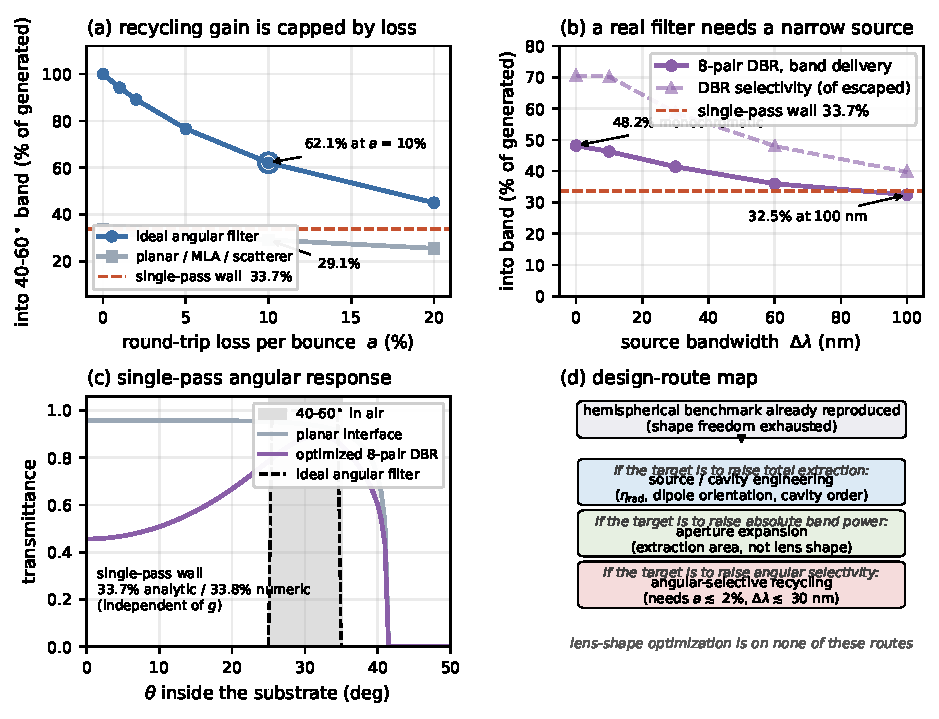
\includegraphics[width=\linewidth]{figures/fig4_recycling_routes.pdf}
\caption{\textbf{The recycling route and the design-route map.} (a) Markov recycling model: power delivered into the 40–60\ensuremath{^\circ} band as a fraction of generated power, versus round-trip loss per bounce $a$, for the ideal angular filter and for the planar non-selective reference. The ideal filter reaches 62.1\% at $a = 10\%$ against 29.1\% for the planar reference, but the two converge as $a$ grows: loss, not filter quality, sets the practical ceiling. (b) Transfer-matrix result for a realizable eight-pair dielectric multilayer: band delivery falls from 48.2\% (monochromatic) to 32.5\% over a 100 nm source bandwidth, crossing back below the single-pass wall. (c) Single-pass angular transmittance of the planar interface, the optimized DBR, and the ideal filter, with the 40–60\ensuremath{^\circ}-in-air acceptance window shaded; the resulting single-pass selectivity wall is 33.7\% analytic / 33.8\% numeric and is independent of the scattering asymmetry $g$. (d) Design-route map: the lever to reach for as a function of the target figure of merit, entered once the hemispherical benchmark has confirmed saturation. Lens-shape optimization appears on none of the three routes.}
\label{fig:4}
\end{figure}


\section{3. Conclusion}

We systematically tested the practical value of freeform shape freedom for manufacturable tiled refractive MLAs on extended OLEDs. Total EQE and each of the four polar bands were optimized as independent single objectives, a weighted-sum sweep and 150 random designs mapped the achievable region, and a separately constrained asymmetric off-axis exploration served as a stress test. Freeform MLAs showed no stable performance gain substantially beyond a hemispherical MLA under identical constraints, and a control that restarted every search at the hemispherical optimum confirmed that this is a property of the design space rather than of the search—the same procedure that returns at most +0.3\% in the two bands at issue recovers +1.0\% to +4.7\% in every objective where a margin genuinely exists: all designs collapsed onto a near-linear efficiency–band-power frontier, and among the most efficient designs the angular composition is fixed to within a few percent regardless of which objective located them. Dedicating the objective to one band does displace that composition—by up to 27\% in selectivity—but costs up to 11\% of total extraction, leaving a net band-power gain of at most 6\% over designs found while pursuing other objectives. This is not a universal claim that the hemisphere is optimal in all optical systems. It is a quantitative finding that when coextensive tiling, an extended source, substrate-mediated lateral mixing, and a fixed radiance/area budget hold simultaneously, the additional freedom purchasable by shape complexity is small. A generality check on two further manufacturable external-film families sharpens this into a bound on how far the angular composition can be moved at all. Across the convex, concave and randomly assembled constructions, and across two averaging conventions within each, every high-efficiency composition falls in the window 0.09–0.11 (0–20\ensuremath{^\circ}), 0.28–0.30 (20–40\ensuremath{^\circ}), 0.34–0.36 (40–60\ensuremath{^\circ}) and 0.21–0.24 (60–80\ensuremath{^\circ}). Randomising lenslet positions and drawing an independent profile for every lenslet leaves the composition inside that window, with a 0.2\% coefficient of variation across disorder realisations; the discrete change to concave lenslets displaces it to the window's edge (0.113/0.303/0.340/0.215) but no further. The angular composition is therefore a property of the platform—extended source, thick substrate, coextensive external film—and not a design variable that shape freedom, array construction, or disorder can command. The saturation statement is made across the three tested manufacturable external-film families, not beyond them; internal, sub-electrode arrays are outside this scope by construction.

The study accordingly does not conclude that freeform MLAs should be abandoned; it supplies a criterion that accelerates the design decision. Once saturation is confirmed against the hemispherical benchmark, the next improvement should be sought not in more lens-shape degrees of freedom but in source/cavity engineering, aperture expansion, or angular-selective recycling. This design-route map applies beyond OLEDs, offering a practical starting point for PeLED, QLED, and micro-LED optical packaging built on extended thin-film sources.

\section{4. Methods}

\subsection{4.1 Trans-scale source model}

Dipole emission in the OLED stack was computed with the CPS formalism. The wavelength- and substrate-angle-resolved intensity $I_{\mathrm{sub}}(\theta,\lambda)$ served as the spectral/angular source of the macroscopic ray tracing. The emitting disc has radius 1 mm; the substrate thickness is 1.295 mm. CPS inputs—material dispersion, dipole orientation, internal radiative efficiency, emission spectrum, layer thicknesses, and wavelength sampling—are collected in Table S1. The same trans-scale pipeline—the CPS dipole microcavity source coupled to LightTools three-dimensional ray tracing—was validated experimentally against fabricated devices in our group's prior publications, in configurations close to the present platform. In ref. \cite{r17}, for OLEDs with an emitting aperture of radius 1 mm, a substrate of thickness 1.4 mm and $n_{\mathrm{sub}} = 1.51$—essentially the geometry of this work—the measured angular emission intensity profiles and current efficiencies of bare, MLA-attached, and structured-outcoupler devices were in good agreement with the trans-scale simulations across all three configurations (Fig.~3 and Table~2 of ref. \cite{r17}; measured maximum EQEs of 35.6\%, 35.4\%, and 48.0\%, respectively). In ref. \cite{r16}, the same pipeline, extended with a diffraction-level bidirectional scattering distribution function, reproduced the measured emission pattern of an inverted-MLA device—cylindrically symmetric output despite the hexagonal lenslet lattice—and its near-Lambertian angular electroluminescence, for a device whose measured EQE reached 58.0\% against 30.5\% for the planar control. The validation therefore covers the source model, the ray-optical treatment of micro-textured exit faces, and both attached and inverted lens constructions, on the same emitter platform and at the same substrate geometry used here.

\subsection{4.2 Lens classes and manufacturing constraints}

The hemispherical reference and the axisymmetric freeform class were compared under one set of constraints: identical lens material, pitch, fill factor, nominal height, boundary continuity, and maximum draft angle. Lenslets of approximately 10 \ensuremath{\mu}m radius are tiled hexagonally over a 25 \ensuremath{\times} 25 mm area on the substrate exit face; the adequacy of this patch size, and the saturating-exponential dependence of total EQE on it, are quantified in Supplementary Table S7. The axisymmetric freeform surface is parameterized by 13 design variables (spline control points, with the radial control points $x_2 \ldots x_6$ constrained monotonic) and implemented as a LightTools native freeform entity. Candidates exhibiting geometric self-intersection, negative thickness, or unmanufacturable draft angles were rejected before optimization. The asymmetric off-axis study of Section 2.4 used a different stack (Ag electrode), an anisotropic emitter cell, and 52 variables, and is reported as a separate exploration, not as part of the controlled benchmark.

\subsection{4.3 Optimization and validation}

Objectives were total EQE, polar-band EQE, or $(\theta,\phi)$-window EQE. Each objective was optimized with MATLAB surrogate-based global optimization (\texttt{surrogateopt}) followed by \texttt{patternsearch} polishing, with multiple independent starts; low-ray search results were re-evaluated with independent high-ray repeats.

The hemisphere-seeded control of Section 2.2 uses the same objective, constraints, geometry and fidelities as the per-band campaign, and differs only in where the search begins. For each arm the 13-variable vector of that arm's hemispherical optimum—the fixed quarter-circle control points together with its own optimized cavity thicknesses and lens height—is placed in the seed set along with eight perturbations drawn within 8\% of each variable's range. The search then proceeds three ways: \texttt{surrogateopt} from that seed set, \texttt{patternsearch} from the surrogate winner, and \texttt{patternsearch} launched directly from the hemisphere point, this last being the most direct test of whether the point is a local optimum in thirteen dimensions. All candidates including the hemisphere itself are screened at search fidelity, and the winner is re-evaluated at final fidelity. The hemisphere baseline is re-measured in the same session rather than taken from the earlier campaign, so that no setting difference between scripts enters the difference; the archived value serves only as a cross-check. An arm counts as improved when the difference exceeds the pooled one-sided 95\% $t$ value at $2(N_{\mathrm{rep}}-1) = 4$ degrees of freedom, i.e. 2.13 standard errors. The one borderline case, 20–40\ensuremath{^\circ} at $t = 2.1$, was settled by re-measuring both stored designs—search excluded—with five fresh repeats each, giving $t = 4.1$ against the five-repeat threshold of 1.86 for a residue of +0.29\%. Note that this control is one-sided by construction: because the hemisphere is among the candidates, the result cannot fall meaningfully below it, and because the winner is selected as the maximum over many noisy search evaluations, the procedure is biased toward reporting a gain. A null result under it is correspondingly conservative. The achievable region was populated with $N = 150$ random feasible designs in addition to the weighted-sum optima at $w \in \{0, 0.25, 0.5, 0.75, 1\}$. Optimization budgets, ray numbers, independent-run counts, feasible-sample counts, and standard deviations are reported in Table S2. Freeform superiority was judged from high-precision means against the hemispherical reference, never from a single best run.

\textbf{Convergence check for the selectivity drift.} Because the correlations between total EQE and band selectivity are small in magnitude for some bands, we verified that they are not sampling artifacts. Twenty designs stratified across the efficiency range were re-evaluated under three progressively stricter conditions: (i) the baseline ray count, (ii) a twenty-fold ray count (200,000 rays) with three independent repeats, and (iii) broadband evaluation over 450–750 nm. The Pearson correlations were stable across all three: $R(0\text{–}20^\circ) = 0.59 \rightarrow 0.61 \rightarrow 0.64$; $R(20\text{–}40^\circ) = 0.67 \rightarrow 0.67 \rightarrow 0.72$; $R(40\text{–}60^\circ) = 0.07 \rightarrow 0.04 \rightarrow 0.05$; $R(60\text{–}80^\circ) = -0.70 \rightarrow -0.71 \rightarrow -0.76$ (Supplementary Table S4). The systematic drift of Section 2.3 is therefore robust against Monte-Carlo noise and narrowband bias.

\subsection{4.4 Angular-selective recycling model}

The external layer is represented by its angular transmission/reflection $T(\theta,\lambda)$ and the reflective electrode by a round-trip loss $a$, combined in a Markov recycling model implemented in Python. The ideal angular filter is defined by $T = 1$ inside the target band and $T = 0$ outside. In the single-pass limit the 40–60\ensuremath{^\circ} band selectivity of non-selective layers is 33.7\% analytically and 33.8\% numerically, and is unchanged over the scattering asymmetry range $g \in [-0.5, +0.5]$ of a two-stream scattering layer. Realizable filters were computed by transfer-matrix calculation of an alternating high/low-index dielectric multilayer (eight pairs). This model is not a proposal of a combined MLA–DBR device; it is a reference calculation separating the saturation of non-selective refractive MLAs from the behavior of selective recycling.

\subsection{4.5 MLA family geometries for the generality test}

The inverted MLA is the concave counterpart of the same freeform profile class: the profile parameterization, constraints, and rejection rules of Methods 4.2 are applied to a concave surface \cite{r16}. The randomly assembled MLA is represented by a pseudo-random supercell: lenslet positions are jittered off the hexagonal lattice by six statistical hyperparameters (fill factor, radius jitter, positional jitter, mean aspect ratio, aspect jitter, and a hemisphere-to-random profile blend), optimized in place of a single lens shape, each lenslet carries an independently drawn random profile from the same parameterized class, and the supercell is tiled periodically over the array area; the construction is statistically equivalent to a random array when the correlation length of the disorder is well below the supercell size (6 \ensuremath{\times} 6 lenslets per supercell on a 141 \ensuremath{\times} 141 height grid, so the disorder correlation length is one lenslet pitch, a sixth of the supercell). The two families follow different protocols, chosen to match what each is being compared against. The inverted family uses the same per-band protocol as the convex benchmark—four single-band arms of 60 surrogate evaluations plus 15 polish steps, with high-precision re-evaluation—so that its natural composition is extracted from a design population generated exactly as the convex one was. The randomly assembled family instead samples 50 random realisations and then optimizes the six assembly statistics, because its design variable is the disorder statistic rather than a lens profile. Budgets and ray counts are reported in Table S2. The random family alone uses reduced sampling—5,000 rays and 16 wavelengths during the search, 10,000 rays and 151 wavelengths for the final re-evaluation—because tracing a supercell costs far more than a single-lens texture. A calibration on one fixed geometry established that this reduction runs 4.3\ensuremath{\times} faster while shifting band selectivity by at most 0.39 percentage points, the same size as the Monte-Carlo spread, so the reported ratios are unaffected (Supplementary Table S3).

\begin{backmatter}

\bmsection{Funding}
[Funding agencies and grant numbers]


\bmsection{Acknowledgments}
[Acknowledgments]


\bmsection{Disclosures}
The authors declare no conflicts of interest.


\bmsection{Data availability}
All result archives underlying the figures and tables of this paper—the
evaluation logs and optima of every optimization campaign
(\texttt{pareto\_front\_result.mat}, \texttt{opt\_4band\_result\_25by25.mat},
\texttt{freeform\_EQEtotal\_result.mat}, \texttt{opt\_hemisphere\_result.mat},
\texttt{opt\_4band\_inverted\_result.mat}, \texttt{stress\_random\_result.mat},
\texttt{warmstart\_hemisphere\_result.mat}, \texttt{reeval\_confirm\_2040\_result.mat},
\texttt{convergence\_check\_result.mat}, \texttt{calibrate\_random\_cost.mat},
\texttt{patch\_convergence\_result.mat}, \texttt{patch\_convergence\_100.mat}) and the recycling-model outputs
(\texttt{angular\_recycling\_result.npz}, \texttt{angular\_recycling\_bandwidth.npz})—are
available from the corresponding author upon reasonable request, together with
the scripts that generated them and the figure-generation script
(\texttt{make\_figures.py}) that reproduces every figure directly from the archives.
Data for the separately constrained asymmetric exploration of Section 2.4 are
available from the corresponding author upon reasonable request. The CPS source
model and LightTools project files require a LightTools license to execute.


\bmsection{Supplemental document}
See Supplement 1 for supporting content.


\end{backmatter}

\begin{thebibliography}{17}

\bibitem{r1} Brütting, W.; Frischeisen, J.; Schmidt, T. D.; Scholz, B. J.; Mayr, C. ``Device Efficiency of Organic Light-Emitting Diodes: Progress by Improved Light Outcoupling." \textit{Phys. Status Solidi A} ``2013", \textit{210}, 44–65.


\bibitem{r2} Yablonovitch, E. ``Statistical Ray Optics." \textit{J. Opt. Soc. Am.} ``1982", \textit{72}, 899–907.


\bibitem{r3} Möller, S.; Forrest, S. R. ``Improved Light Out-Coupling in Organic Light Emitting Diodes Employing Ordered Microlens Arrays." \textit{J. Appl. Phys.} ``2002", \textit{91}, 3324–3327.


\bibitem{r4} Wrzesniewski, E.; et al. ``Enhancing Light Extraction in Top-Emitting Organic Light-Emitting Devices Using Molded Transparent Polymer Microlens Arrays." \textit{Small} ``2012", \textit{8}, 2647–2651. \url{https://doi.org/10.1002/smll.201102662}


\bibitem{r5} Qu, Y.; Kim, J.; Coburn, C.; Forrest, S. R. ``Efficient, Nonintrusive Outcoupling in Organic Light Emitting Devices Using Embedded Microlens Arrays." \textit{ACS Photonics} ``2018", \textit{5}, 2453–2458. \url{https://doi.org/10.1021/acsphotonics.8b00255}


\bibitem{r6} Kim, S.; Shin, J. M.; Lee, J.; Park, C.; Lee, S.; Park, J.; Seo, D.; Park, S.; Park, C. Y.; Jang, M. S. ``Inverse Design of Organic Light-Emitting Diode Structure Based on Deep Neural Networks." \textit{Nanophotonics} ``2021", \textit{10}, 4533–4541. \url{https://doi.org/10.1515/nanoph-2021-0434}


\bibitem{r7} Ni, Y.; Feng, D.; Ma, D. ``Design of Freeform Microlens Arrays with Prescribed Luminance Distributions for MicroLED Optical Packaging." \textit{Appl. Opt.} ``2025", \textit{64}, 7875–7884. \url{https://opg.optica.org/ao/abstract.cfm?uri=ao-64-27-7875}


\bibitem{r8} Buhl, M.; et al. ``Resonance-Based Directional Light Emission from Organic Light-Emitting Diodes." \textit{Adv. Photonics Res.} ``2023", \textit{4}, 2200143. \url{https://doi.org/10.1002/adpr.202200143}


\bibitem{r9} Abdelkhalik, M. S.; Garcia-Santiago, X.; van Raaij, T.-J.; López, T.; Berghuis, A. M.; de Jong, L. M. A.; Gómez Rivas, J. ``Enhanced and Directional Electroluminescence from MicroLEDs Using Metallic or Dielectric Metasurfaces." \textit{Commun. Eng.} ``2025", \textit{4}, 63. \url{https://doi.org/10.1038/s44172-025-00401-w}


\bibitem{r10} Winston, R.; Jiang, L.; Ricketts, M. ``Nonimaging Optics: A Tutorial." \textit{Adv. Opt. Photon.} ``2018", \textit{10}, 484–511.


\bibitem{r11} Rau, U. ``Reciprocity Relation between Photovoltaic Quantum Efficiency and Electroluminescent Emission of Solar Cells." \textit{Phys. Rev. B} ``2007", \textit{76}, 085303.


\bibitem{r12} Xiang, C.; Koo, W.; So, F.; Sasabe, H.; Kido, J. ``A Systematic Study on Efficiency Enhancements in Phosphorescent Green, Red and Blue Microcavity Organic Light-Emitting Devices." \textit{Light: Sci. Appl.} ``2013", \textit{2}, e74. \url{https://doi.org/10.1038/lsa.2013.30}


\bibitem{r13} Song, J.; et al. ``Lensfree OLEDs with over 50\% External Quantum Efficiency via External Scattering and Horizontally Oriented Emitters." \textit{Nat. Commun.} ``2018", \textit{9}, 3207. \url{https://doi.org/10.1038/s41467-018-05671-x}


\bibitem{r14} Liao, P.-H.; Lee, W.-K.; Lee, C.-C.; Huang, C.-W.; Wen, S.-W.; Chen, Y.-T.; Chen, C.-C.; Lin, W.-Y.; Kwak, B. L.; Visser, R. J.; Wu, C.-C. ``Using Angle-Selective Optical Film to Enhance the Light Extraction of a Thin-Film Encapsulated 3D Reflective Pixel for OLED Displays." \textit{Opt. Express} ``2022", \textit{30}, 46435–46449. \url{https://doi.org/10.1364/OE.477797}


\bibitem{r15} Kim, H.-J.; et al. ``High Efficient OLED Displays Prepared with the Air-Gapped Bridges on Quantum Dot Patterns for Optical Recycling." \textit{Sci. Rep.} ``2017", \textit{7}, 43063. \url{https://doi.org/10.1038/srep43063}


\bibitem{r16} Kim, J.; Kim, E.; Park, J.; Song, J.; Kim, S.; Moon, H.; Yoo, S. ``Toward Near-Foldable Surface Light Sources with Ultimate Efficiency: Ultrathin Substrates Embedded with Micron-Scale Inverted Lens Arrays." \textit{ACS Photonics} ``2023", \textit{10}, 1775–1782. \url{https://doi.org/10.1021/acsphotonics.3c00017}


\bibitem{r17} Kim, M.; Kim, J.; Yoo, S. ``Near-Planar Light Outcoupling Structures with Finite Lateral Dimensions for Ultra-Efficient and Optical Crosstalk-Free OLED Displays." \textit{Nat. Commun.} ``2025", \textit{16}, 11606. \url{https://doi.org/10.1038/s41467-025-66538-6}


\end{thebibliography}

\end{document}